
\leo{We have asymptotic results on total variation distance going to 0, and non-asymptotic bound when $\lambda>m>0$, if  $\int_{\mc D} \pi_{\mc R}(\theta)d\theta>0$. But the non-asymptotic bound fails if  $\int_{\mc D} \pi_{\mc R}(\theta)d\theta=0$. If we are to bound distance between two measures, we might need to switch to Wasserstein distance with Eucledean norm in the whole section.}

We now study the properties of the extrinsic prior and posterior. One important task is to quantify the difference between extrinsic and intrinsic ones. Due to similar reasoning for prior and posterior, we use some general notation. Let $\pi_{\mc R}(\theta)$ be an unnormalized density in $\mc R$, which is $\pi_{0,\mc R}(\theta)$ when studying prior and $L(y;\theta)\pi_{0,\mc R}(\theta)$ when studying posterior; $\Pi(.)$ and $\tilde\Pi(.)$ to represent the measures under intrinsic and extrisic methods associated with either prior or posterior distribution. 

We first explore the case case in \eqref{exact_prior1} and  \eqref{exact_posterior1}, where $\int_{\mc D} \pi_{\mc R}(\theta)d\theta>0$.

%distance between extrinsic and intrinsic
\begin{remark}
Let $M_1= \int_{\mc R} \pi_{0,\mc R}(\theta) \mathbbm{1}_{\theta\in \mc D} d\theta$ and $M_2 = \int_{\mc R} \pi_{\mc R}(\theta) \mc K(\theta;\mc D)d\theta$, when $M_1>0$, the total variation distance between the measures of extrinsic and intrinsic distributions is
$$||\Pi(.), \tilde{\Pi}(.) ||_{TV} = 1 - \frac{M_1}{M_2} \le \frac{\int_{\mc R \setminus \mc D} \pi_{\mc R}(\theta) \mc K(\theta;\mc D)d\theta}{M_1}.$$
\end{remark}
proof:
{Via definition of total variation distance and $\mc K(\theta;\mc D)=1$ when $\theta\in\mc D$.}

Using exponential smoothing function $\mc K(\theta; D) = \prod_{k=1}^m \exp( -v_k(\theta)/\lambda_k)$, as all $\lambda_k \rightarrow 0$, the total variation $||\Pi(.), \tilde{\Pi}(.) ||_{TV} \rightarrow 0$, if $\int_{\mc R} \pi_{\mc R}(\theta) d\theta<\infty$. This is a direct result of dominated convergence theorem and $\mc K(\theta; \mc D)\le 1$.


With some mild assumptions, we further quantify the non-asymptotic rate. Letting $\lambda = \sup_k \lambda_k$, $M= \int_{\mc R \setminus \mc D} \pi_{\mc R}(\theta) d\theta<\infty$. As a linear combination of measurable functions, $v(\theta)=\lambda\sum_{k=1}^m\frac{ v_k(\theta)}{\lambda_k}$ is measurable. Let $f(v)$ be the density of $v(\theta)$.

\begin{remark}
\label{convergence_rate}
If there exists a $t<\infty$ such that $f(v) < \infty$, for any $t>0$,
$$\int_{\mc R \setminus \mc D} {\pi_{\mc R}(\theta)} \prod_{k=1}^m \exp( -v_k(\theta)/\lambda_k) d \theta \le 
 {M} \exp(-\frac{t}{\lambda}) + {M} \sup_{t^*\in(0,t)} {f(t^*)}\lambda 
$$
\end{remark}
\aki{The density of $v(\theta)$ crucially depends on the level set of $v(\theta)$ and is a pretty complicated (i.e.\ intractable) object in general.}

\leo{The point is that if the measure of $v$ is Lipschitz in a $t$-ball of $\mc D$, then $\sup_{t^*\in(0,t)} {f(t^*)}$ is bounded; $\exp(-\frac{t}{\lambda})$ goes to $0$ faster than $\lambda$, so the whole term goes to $0$ in $\mc O(\lambda)$.}

\begin{proof}[Proof]
\begin{equation}
\begin{aligned}
\frac{1}{M}\int_{\mc R \setminus \mc D} {\pi_{\mc R}(\theta)} \prod_{k=1}^m \exp( -v_k(\theta)/\lambda_k) d \theta = & 
\mathbb{E} \exp(- \frac{v}{\lambda}) \\
= & \mathbb{E} \mathbbm{1}_{(0,t)} \exp(- \frac{v}{\lambda}) +  \mathbb{E} \mathbbm{1}_{(t,\infty)} \exp(- \frac{v}{\lambda}) \\
\le & \int_0^t f(v) \exp(- \frac{v}{\lambda}) dv + \exp(-\frac{t}{\lambda}) \\
\le & \sup_{t^*\in(0,t)} f(t^*) \int_0^t \exp(- \frac{v}{\lambda}) dv + \exp(-\frac{t}{\lambda}) \\
= & \sup_{t^*\in(0,t)} f(t^*)  \lambda (1- \exp(-t/\lambda)) + \exp(-\frac{t}{\lambda}) \\
\le  & \sup_{t^*\in(0,t)} f(t^*)  \lambda  + \exp(-\frac{t}{\lambda}) \\
\end{aligned}
\end{equation}
Rearranging terms yields the result.
\end{proof}

For $\lambda$ close to $0$, the extrinsic measure approaches intrinsic one in total varation distance in $O(\lambda)$. This rate is quantified under very general assumption. We expect it can be sharpened under special cases.

We now examine the second case in \eqref{exact_prior2} and \eqref{exact_posterior2} where ${ \int_{\mc D} \pi_{\mc R}(\theta)d\theta }=0$.


\begin{remark}
If both $\lim_{r\rightarrow 0^+} \frac{\int_{B} \pi_{\mc R}(\theta) \mathbbm{1}_{\theta\in \mc D_r} d\theta}{ \int_{\mc D_r} \pi_{\mc R}(\theta)d\theta }$ and $ \lim_{r\rightarrow 0^+}\frac{\int_{B} \pi_{\mc R}(\theta) \mc K({\theta; \mc D_r}) d\theta}{ \int_{\mc R} \pi_{\mc R}(\theta)  \mc K({\theta; \mc D_r}) d\theta }  $ converge uniformly in $B$, the total variation distance between the measures of extrinsic and intrinsic distribution

\begin{equation}
	\begin{aligned}
	||\Pi(.), \tilde{\Pi}(.) ||_{TV}
	= &\sup_{B} ||\Pi(B)- \tilde{\Pi}(B)||\\
	= & \sup_{B}|| \lim_{r\rightarrow 0^+} \frac{\int_{B} \pi_{\mc R}(\theta) \mathbbm{1}_{\theta\in \mc D_r} d\theta}{ \int_{\mc D_r} \pi_{\mc R}(\theta)d\theta }-  \lim_{r\rightarrow 0^+}\frac{\int_{B} \pi_{\mc R}(\theta) \mc K({\theta; \mc D_r}) d\theta}{ \int_{\mc R} \pi_{\mc R}(\theta)  \mc K({\theta; \mc D_r}) d\theta } || \\
	= & \lim_{r\rightarrow 0^+} \sup_{B}|| \frac{\int_{B} \pi_{\mc R}(\theta) \mathbbm{1}_{\theta\in \mc D_r} d\theta}{ \int_{\mc D_r} \pi_{\mc R}(\theta)d\theta }-  \frac{\int_{B} \pi_{\mc R}(\theta) \mc K({\theta; \mc D_r}) d\theta}{ \int_{\mc R} \pi_{\mc R}(\theta)  \mc K({\theta; \mc D_r}) d\theta } || \\
	=& \lim_{r\rightarrow 0^+}  \frac{\int_{\mc R \setminus \mc \mc D_r} \pi_{\mc R}(\theta) \mc K(\theta;\mc D_r)d\theta}{\int_{\mc R \setminus \mc D} \pi_{\mc R}(\theta) \mc K(\theta;\mc D_r)d\theta}.
	\end{aligned}
\end{equation}
\end{remark}

 Let $g(r,\lambda)=
\frac{\int_{\mc R \setminus \mc  D_r} \pi_{\mc R}(\theta) \mc K(\theta;\mc D_r)d\theta}{\int_{\mc R \setminus \mc D} \pi_{\mc R}(\theta) \mc K(\theta;\mc D_r)d\theta}$, using exponential smoothing function and $\lambda = \sup_k\lambda_k$, $\lim_{\lambda\rightarrow 0^+}g(r,\lambda)=0$ pointwise in $r$. And we have  $||\Pi(.), \tilde{\Pi}(.) ||_{TV}\le \lim_{r\rightarrow 0^+}\frac{{M_r} \exp(-\frac{t}{\lambda}) + {M_r} \sup_{t^*\in(0,t)} {f(t^*)}\lambda }{\int_{\mc R  \setminus \mc D} \pi_{\mc R}(\theta) \mc K(\theta;\mc D_{r})d\theta}$ assuming $M_r= \int_{\mc R \setminus \mc D_{r}} \pi_{\mc R }(\theta) d\theta<\infty$. For every $r$, there is a small $\lambda$ to make the total variation distance arbitrarily small. However, with $\lambda=\lambda_0$ fixed and non-negligble, $\lim_{r\rightarrow 0^+}g(r,\lambda)=1$. This is due to the over-sensitivity of total variation distance in comparing continuous and degenerate distributions. Therefore, to quantify distance with non-zero $\lambda$, we consider general Wasserstein distance:

$$W_p(\Pi,\tilde\Pi)=\left(\underset{\gamma\in \Gamma(\Pi,\tilde\Pi)}{\inf}\int \text{dist}(x,y)^p d\gamma(x,y)\right)^{1/p}$$
 where $ \text{dist}(x,y)$ is the metric on $\mc R$ and $\Gamma(\Pi,\tilde\Pi)$ the set of couplings of $\Pi$ and $\tilde\Pi$. The total variation distance is a special case with $p=1$ and $d(x,y)= \mathbbm{1}_{x \neq y}$. Instead we consider Eucledean norm $\text{dist}(x,y)=||x-y||$.


{\bf Example 1C: Distance between intrinsic and extrinsic distributions} 

We continue in Example 1, denoting the bivariate Gaussian distribution obtained extrinsically as $\No(\mu_\lambda, \Sigma_\lambda)$, the intrinsic one can be viewed as $\No(\mu_0, \Sigma_0)$. The Wasserstein distance between the intrinsic and extrinsic distributions in Example 1 \citep{dowson1982frechet} is $W_2 (\Pi,\tilde\Pi)= \left( ||\mu_\lambda - \mu_0||_2^2+ \text{tr}(\Sigma_\lambda+\Sigma_0- 2 (\Sigma_\lambda^{1/2}  \Sigma_0 \Sigma_\lambda^{1/2})^{1/2}) \right)^{1/2} $. Figure~\ref{two_normal_wass} plots $W_2$ under different values of $\lambda$, with $W_2\approx 0$ with $\lambda=10^{-3}$.



\begin{figure}[H]
\centering
   \begin{subfigure}[b]{0.45\textwidth}
    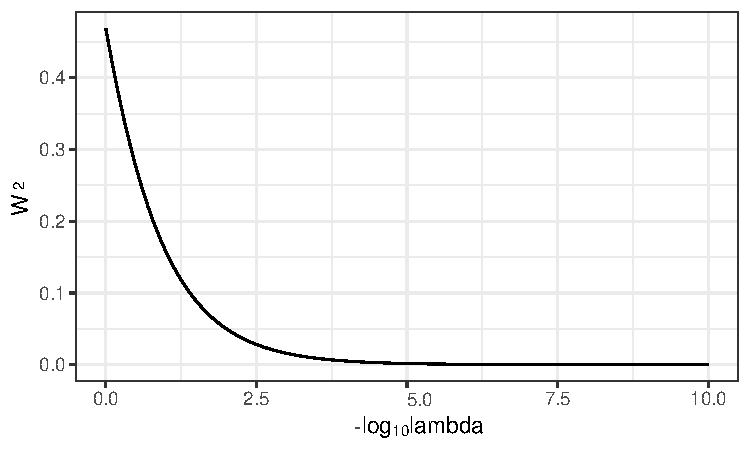
\includegraphics[width=1\textwidth]{two_normal_wass.pdf}
	\end{subfigure}
\caption{Wasserstein distance of 2nd order $W_2$ between the intrinsic and extrinsic prior for two normal random variables under sum constraint. $W_2$ declines rapidly as $\lambda$ (shown as $-\log_{10}(\lambda)$) decreases.}
\label{two_normal_wass}
\end{figure}


\subsection{\textcolor{red}{Approximation Error (Aki's proposal)}}

\aki{The convergence in total variation is too strong, so I propose something like below.}

\leo{Aki, I like your use of Feder's co-area forumula, can we get some non-asympotic result when $\lambda>m$ (away from 0)?}

\aki{A non-asymptotic result should hold as long as we put the right assumptions on $f(\theta)$. I'd think the key assumption is $\nabla f(\theta)$ to be a unit vector orthogonal to $\mc D$ whenever $\theta \in \mc D$. I don't know how to rigorously estimate the difference in the integrals over the surface $f^{-1}(0)$ and $f^{-1}(\alpha)$, however. (I can do it if $\mc D$ is a compact manifold, I think.) We may need help from an expert in geometric methods.}



\newcommand{\tilpi}{\tilde{\pi}}

We establish that the inference based on an intrinsic prior is well approximated by the one based on an extrinsic prior for sufficiently small $\lambda$. In particular, for a posterior summary of interest $g(\theta)$, we have $\mathbb{E}_{\tilpi_{\mc D, \lambda}}[g(\theta)] \to \mathbb{E}_{\pi_{\mc D}}[g(\theta)]$ as $\lambda \to 0$ provided $g(\theta)$ is continuous and integrable under the extrinsic posterior for some $\lambda < \infty$. In case the constraint takes the form $\mc D = \{f(\theta) = 0\}$ and the extrinsic posterior is given by $\tilpi_{\mc D, \lambda}(\theta) = \pi_{\mc R}(\theta) \exp(- \lambda^{-1} |f(\theta)|) \, / \, Z_\lambda$, the proof is as follows. \aki{From the proof, it appears that we also need to choose the constraint so that  $\| \nabla f \| \equiv 1$ on $\mc D$. This makes sense from geometric intuition too, I think.}

\leo{I'm not sure if $\| \nabla f \| \equiv 1$ is easy to have, for example how to scale $f(x,y)=x^3+y^3 -1$ uniformly to have $\| \nabla f \| \equiv 1$?}
\begin{proof}[Proof]
	By the co-area formula of Federer \citep{diaconis2013manifold}, we have
	\begin{equation}
	\lambda^{-1} Z_\lambda
	= \lambda^{-1} \int_{\mathbb{R}^d} \pi_{\mc R}(\theta) \exp(- \lambda^{-1} |f(\theta)|)  d \theta
	= \int_{-\infty}^{\infty}  \left[ \int_{f^{-1}(\alpha)} \frac{ \pi_{\mc R}(\theta) }{ \| \nabla f(\theta) \| } \mathcal{H}^{d-1}(d \theta) \right]  \lambda^{-1} \exp(- \lambda^{-1} |\alpha| ) d \alpha
	\end{equation}
	where $\mathcal{H}^{k}(d \theta)$ denotes a $k$-dimensional Hausdorff measure. Since the measure $\exp(- \lambda^{-1} |\alpha| ) d \alpha$ concentrates around $\alpha = 0$ as $\lambda \to 0$, we obtain
	\begin{equation}
	\lim_{\lambda \to 0} \lambda^{-1} Z_\lambda
	= \int_{f^{-1}(0)} \frac{ \pi_{\mc R}(\theta) }{ \| \nabla f(\theta) \| } \mathcal{H}^{d-1}(d \theta) 
	= \int_{f^{-1}(0)} \pi_{\mc D}(d \theta)
	\end{equation}
	by the assumption $\| \nabla f(\theta) \|  = 1$ and the fact that $\pi_{\mc D}(d \theta)$ coincides with the conditional density of $\pi_{\mc R}(\theta)$ on $\mc D$. Also by the co-area formula,
	\begin{equation}
	\int_{\mathbb{R}^d} g(\theta) \pi_{\mc R}(\theta) \exp(- \lambda^{-1} |f(\theta)|)  /  Z_\lambda d \theta
	= \int_{-\infty}^{\infty}  \left[ \int_{f^{-1}(\alpha)} \frac{ g(\theta) \pi_{\mc R}(\theta) }{ \| \nabla f(\theta) \| } \mathcal{H}^{d-1}(d \theta) \right]  \exp(- \lambda^{-1} |\alpha| )  /  Z_\lambda d \alpha
	\end{equation}
	Again, since the measure $\exp(- \lambda^{-1} |\alpha| ) d \alpha$ concentrates around $\alpha = 0$ as $\lambda \to 0$, we obtain
	\begin{equation}
	\lim_{\lambda \to 0} \int_{\mathbb{R}^d} g(\theta) \pi_{\mc R}(\theta) \exp(- \lambda^{-1} |f(\theta)|)  /  Z_\lambda d \theta
	= \int_{f^{-1}(0)} \frac{ g(\theta) \pi_{\mc R}(\theta) }{ \| \nabla f(\theta) \| } d \mathcal{H}^{d-1}(\theta) 
	= \frac{\int_{f^{-1}(0)} g(\theta) \pi_{\mc D}(d \theta)}{\int_{f^{-1}(0)} \pi_{\mc D}(d \theta)} \qedhere
	\end{equation}
\end{proof}
